\chapter{Технологический раздел}


В данном разделе будут представлены средства реализации, реализация приложения, тестирование и интерфейс приложения.


\section{Средства реализации}
\subsection{Выбор языка}
Для разработки был выбран язык Golang. Данный выбор обусловлен следующими возможностями языка:
\begin{itemize}
	\item Возможность шифрования данных \cite{golang_crypt}
	\item Возможность взаимодействия с выбранными СУБД \cite{golang_dbms}
	\item Возможность удобного тестирования ПО \cite{golang_testing}
	\item Возможность работы с JWT-токенами \cite{golang_jwt}
\end{itemize}

\subsection{Выбор СУБД}
В аналитическом разделе был сделан выбор в пользу реляционной модели БД.
Соответственно, выбор СУБД будет производиться с учетом работы с реляционными моделями.
Наиболее популярные и свободно~--~распространяемые СУБД: MySQL, MariaDB, PostgreSQL, Firebird.
Критериями для выбора являются:
\begin{itemize}
	\item имеющийся опыт работы с выбранной СУБД;
	\item наличие документации выбранной СУБД;
	\item поддержка со стороны комьюинити;
	\item поддержка триггер механизмов;
	\item предоставление процедурного языка.
\end{itemize}

Всем этим требованием удовлетворяет СУБД PostregSQL.

\section{Реализация процедур}
Реализация процедур, используемых во время работы алгоритма добавления брони представлены на листингах \ref{lst:is_intersect} --- \ref{lst:is_reserve}.
\newline
\begin{lstlisting}[label=lst:is_reserve]
create or replace function is_reserve(userId integer,
									roomId integer,
									producerId integer,
									instrumentalistId integer,
									startTime timestamp,
									endTime timestamp) returns integer language plpgsql as $$
declare
	count integer;
begin
	select count(*) into count
	from reserve
	where (user_id = userId or
		room_id = roomId or
		producer_id = producerId or
		instrumentalist_id = instrumentalistId) and 
			is_intersect(reserve.start_time,
						reserve.end_time,
						startTime,
						endTime);

	return count;
end;
$$;
\end{lstlisting}
\captionof{figure}{Реализация алгоритма проверки занятости}
\newpage

\begin{lstlisting}[language=sql, label=lst:is_intersect]
create or replace function is_intersect(reserveStartTime timestamp, 
										reserveEndTime timestamp,
										choosenStartTime timestamp,
										choosenEndTime timestamp) returns boolean language plpgsql as $$
declare
	ans boolean;
begin
	ans = false;
	if ((choosenStartTime >= reserveStartTime and choosenStartTime < reserveEndTime) or
	(choosenEndTime <= reserveEndTime and choosenEndTime > reserveStartTime) or
	(choosenStartTime <= reserveStartTime and choosenEndTime >= reserveEndTime)) then
		ans = true;
	end if;
	return ans;
end;
$$;
\end{lstlisting}
\captionof{figure}{Реализация алгоритма проверки пересечения времени}

\section{Реализация приложения}

Приложение было реализовано на основе принципа чистой архитектуры.
Приложение было разделено на несколько компонентов: Service, Repository и Model.
\begin{itemize}
	\item Service --- отвечает за бизнес~--~логику приложения;
	\item Repository --- отвечает за работу с хранилищем данных;
	\item Model --- отвечает за хранение сущностей приложения и перенос данных между компонентами приложения.
\end{itemize}
Именно в компоненте Repository хранятся заготовленные запросы к БД, работающие с помощью библиотеки pgx --- драйвера PostgreSQL для языка Golang. 



\section{Тестирование}
Для тестирования системы использовались интеграционные тесты и модульные тесты.

Для проверки use--case методов использовались интеграционные тесты.
Для создания тестов использовалась библиотека testing для Golang~\cite{golang_testing}.
Созданные модульные тесты полностью покрывают все методы.

Для тестирования используемых SQL запросов были использованы две библиотеки.
С помощью библиотеки testing для Golang~\cite{golang_testing} были созданы непосредственно тесты, а с помощью библиотеки testcontainers~\cite{golang_testcontainers} поднимались контейнеры Docker~\cite{docker}, которые, с использованием ранее заготовленных миграций, создавали необходимое состояние БД в контейнере под тесты.
Данный подход позволяет проводить тестирование независимо от основной рабочей БД.

После успешной подготовки, было выполнено модульное и интеграционное тестирование, которое обеспечивает полное покрытие используемых методов, которые, в свою очередь, содержат SQL запросы.

Все тесты были пройдены успешно.

В приложении А приведены код и результат работы тестирования. 

\section{Интерфейс приложения}
Интерфейс приложения был создан с помощью сторонней библиотеки tview~\cite{golang_tview}.
Данная библиотека позволяет создавать отдельные страницы для работы с пользователем и дает возможность перемещаться между ними. 

\subsection{Интерфейс гостя}

При запуске, приложение считает любого пользователя гостем. 
Гостю предлагается либо посмотреть уже существующие брони, либо авторизоваться.

Первая страница приложения представлена на рисунке~\ref{img:auth}.

%\begin{center}
%	\centering
%	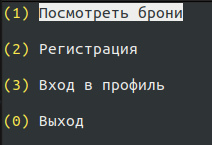
\includegraphics[height=0.2\textheight]{inc/img/auth.png}
%	\captionof{figure}{Страница с авторизацией}
%	\label{img:auth}
%\end{center}


\includeimage
{auth} % Имя файла без расширения (файл должен быть расположен в директории inc/img/)
{f} % Обтекание (с обтеканием)
{H} % Положение рисунка (см. wrapfigure из пакета wrapfig)
{0.4\textwidth} % Ширина рисунка
{Страница с авторизацией} % Подпись рисунка



\subsection{Интерфейс авторизованного пользователя}
После успешной регистрации или авторизации пользователь переходит на основную страницу, на которой можно создать бронь, удалить или посмотреть уже созданные.
Также можно выйти из профиля или приложения.

Основная страница приложения представлена на рисунке~\ref{img:main_client}.

%\begin{center}
%	\centering
%	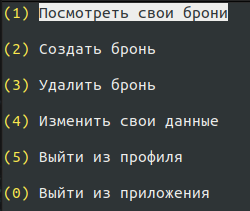
\includegraphics[height=0.3\textheight]{inc/img/main_client.png}
%	\captionof{figure}{Основная страница}
%	\label{img:main_client}
%\end{center}


\includeimage
{main_client} % Имя файла без расширения (файл должен быть расположен в директории inc/img/)
{f} % Обтекание (с обтеканием)
{H} % Положение рисунка (см. wrapfigure из пакета wrapfig)
{0.4\textwidth} % Ширина рисунка
{Основная страница} % Подпись рисунка



При нажатии на кнопку <<Создать бронь>> откроется меню, в котором необходимо будет выбрать желаемую студию и внести период брони.
После нажатия на кнопку <<Продолжить>> система автоматически подберет все возможные варианты атрибутов для брони и предоставит выбор на следующей странице.
После того, как пользователь сделает выбор и нажмет кнопку <<Создать бронь>>, то в соответствующую табличку в БД добавится новый кортеж.

Первая и вторая страница создания брони представлены на рисунке~\ref{img:validate} и~\ref{img:create_reserve}.

%\begin{center}
%	\centering
%	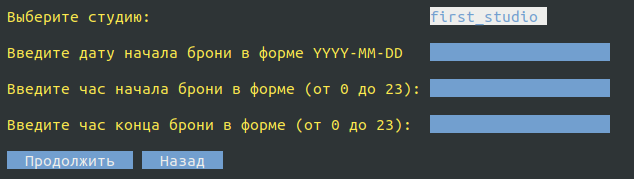
\includegraphics[height=0.105\textheight]{inc/img/validate.png}
%	\captionof{figure}{Первая страница для создания брони брони}
%	\label{img:validate}
%\end{center}

\includeimage
{validate} % Имя файла без расширения (файл должен быть расположен в директории inc/img/)
{f} % Обтекание (с обтеканием)
{H} % Положение рисунка (см. wrapfigure из пакета wrapfig)
{0.65\textwidth} % Ширина рисунка
{Первая страница для создания брони брони} % Подпись рисунка


%\begin{center}
%	\centering
%	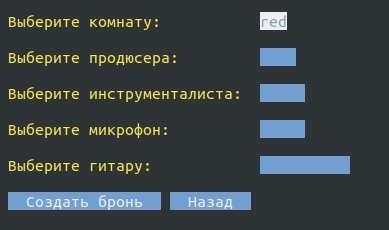
\includegraphics[height=0.22\textheight]{inc/img/create_reserve.png}
%	\captionof{figure}{Вторая страница для создания брони брони}
%	\label{img:reserve_create}
%\end{center}


\includeimage
{create_reserve} % Имя файла без расширения (файл должен быть расположен в директории inc/img/)
{f} % Обтекание (с обтеканием)
{H} % Положение рисунка (см. wrapfigure из пакета wrapfig)
{0.4\textwidth} % Ширина рисунка
{Вторая страница для создания брони брони} % Подпись рисунка


На рисунке~\ref{img:delete_reserve} представлена страница для снятия брони.
Пользователю необходимо выбрать из выпадающего меню нужную дату и нажать кнопку <<Снять бронь>>.

%\begin{center}
%	\centering
%	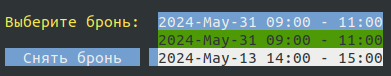
\includegraphics[height=0.07\textheight]{inc/img/delete_reserve.png}
%	\captionof{figure}{Страница для снятия брони}
%	\label{img:delete_reserve}
%\end{center}

\includeimage
{delete_reserve} % Имя файла без расширения (файл должен быть расположен в директории inc/img/)
{f} % Обтекание (с обтеканием)
{H} % Положение рисунка (см. wrapfigure из пакета wrapfig)
{0.5\textwidth} % Ширина рисунка
{Страница для снятия брони} % Подпись рисунка


Страница, содержащая созданные пользователем брони и информацию о них, представлена на рисунке~\ref{img:my_reserves}.
 

%\begin{center}
%	\centering
%	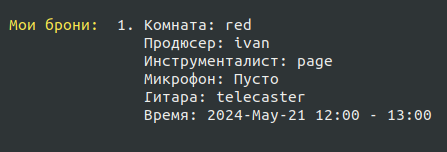
\includegraphics[height=0.12\textheight]{inc/img/my_reserves.png}
%	\captionof{figure}{Страница броней пользователя}
%	\label{img:my_reserves}
%\end{center}

\includeimage
{my_reserves} % Имя файла без расширения (файл должен быть расположен в директории inc/img/)
{f} % Обтекание (с обтеканием)
{H} % Положение рисунка (см. wrapfigure из пакета wrapfig)
{0.5\textwidth} % Ширина рисунка
{Страница броней пользователя} % Подпись рисунка


\subsection{Интерфейс администратора}
Основное меню администратора продемонстрировано на рисунке~\ref{img:main_admin}.
Из него можно перейти в другие меню для добавления, удаления или изменения атрибутов.

%\begin{center}
%	\centering
%	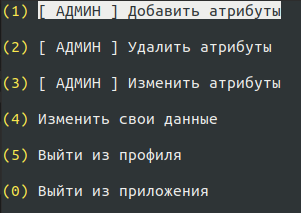
\includegraphics[height=0.2\textheight]{inc/img/main_admin.png}
%	\captionof{figure}{Основная страница администратора}
%	\label{img:main_admin}
%\end{center}

\includeimage
{main_admin} % Имя файла без расширения (файл должен быть расположен в директории inc/img/)
{f} % Обтекание (с обтеканием)
{H} % Положение рисунка (см. wrapfigure из пакета wrapfig)
{0.45\textwidth} % Ширина рисунка
{Основная страница администратора} % Подпись рисунка

Каждая из первых трех функций на странице администратора содержит еще дополнительные меню.
В каждом из меню необходимо выбрать атрибут, над которым будет проведено выбранное действие.

Пример данного меню представлен на рисунке~\ref{img:add_menu}.

%\begin{center}
%	\centering
%	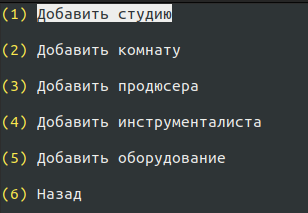
\includegraphics[height=0.23\textheight]{inc/img/add_menu.png}
%	\captionof{figure}{Меню для добавления}
%	\label{img:add_menu}
%\end{center}

\includeimage
{add_menu} % Имя файла без расширения (файл должен быть расположен в директории inc/img/)
{f} % Обтекание (с обтеканием)
{H} % Положение рисунка (см. wrapfigure из пакета wrapfig)
{0.45\textwidth} % Ширина рисунка
{Меню для добавления} % Подпись рисунка


\section*{Вывод}
В данном разделе были представлены средства реализации, реализация приложения, тестирование и интерфейс приложения.
